%++++++++++++++++++++++++++++++++++++++++
% Don't modify this section unless you know what you're doing!
\documentclass[letterpaper,12pt]{article}
\usepackage{tabularx} % extra features for tabular environment
\usepackage{amsmath}  % improve math presentation
\usepackage{graphicx} % takes care of graphic including machinery
\usepackage[margin=1in,letterpaper]{geometry} % decreases margins
\usepackage{cite} % takes care of citations
\usepackage[final]{hyperref} % adds hyper links inside the generated pdf file
\usepackage[numbib,nottoc]{tocbibind}
\usepackage{float}
\usepackage{longtable}
\usepackage{listings}
\usepackage{textgreek}
\usepackage[utf8]{inputenc}
\hypersetup{
	colorlinks=true,       % false: boxed links; true: colored links
	linkcolor=blue,        % color of internal links
	citecolor=blue,        % color of links to bibliography
	filecolor=magenta,     % color of file links
	urlcolor=blue         
}
%++++++++++++++++++++++++++++++++++++++++


\begin{document}

\title{ADMT 2018 - Project report}
\author{Group 02: Andreas Vieider (13177) \& Laurin Stricker (13412)}
\date{\today}
\maketitle

% \begin{abstract}

% \end{abstract}


\section{Introduction}

The domain of our fictional company is the one of furniture production and retail. The company is located in the province of Bolzano and has several showrooms in the area and one production center.

\subsection{Business processes}

\subsubsection{CRM - Showroom visit}

One CRM process is the collection of data about visitors at the different showrooms. A visitor can either be one who is just looking around without intention of buying anything (Seeleute), a future potential customer or an already existing customer. A visit can lead to an order.

Business questions:
\begin{itemize}
        \item Which is the best running showroom (most visitors, most orders, etc.)
        \item Where are the customers from (with different granularity)
        \item Which department are the customers the most interested in
        \item Compare the number of visitors to the number of customers for a time period and/or showroom
\end{itemize}

\subsubsection{Production}

The company logs every step in the production process, especially duration, defects and machine failures.

Business questions:
\begin{itemize}
        \item What is the average time to produce a particular product
        \item Which is the product with the highest/lowest quality
        \item How much effort/time is spent per production stage, product category
				\item What is the production cost of a product
\end{itemize}

\section{Conceptual Design}

\begin{longtable}{p{3cm}p{6cm}p{4cm}}
        \caption{Fact table} \\
        \hline \\
        Fact & Dimensions & Measures \\
        \hline \\
        \endfirsthead \\
        Fact & Dimensions & Measures \\
        \endhead \\
        \hline \\
        Showroom visit & Date, Showroom, Visitor, Order, Detail, Department, Sales representative & Duration (AVG), Amount of people (SUM, AVG) \\
        \hline \\
        Production & Start Date, End date, Product, Production Stage, Machine, Quality control, Operator & Duration (AVG), Raw material cost (AVG) \\
        \hline \\
\end{longtable}

\begin{figure}[H] 
        \centering
        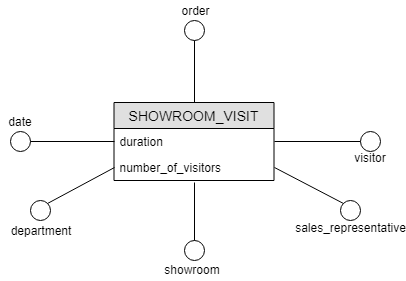
\includegraphics[scale=0.65]{../images/DFM_Showroom_Simple.png}
        \caption{
                \label{fig:showroom}  
                DFM of the showroom visit
        }
\end{figure}

\begin{figure}[H] 
        \centering
        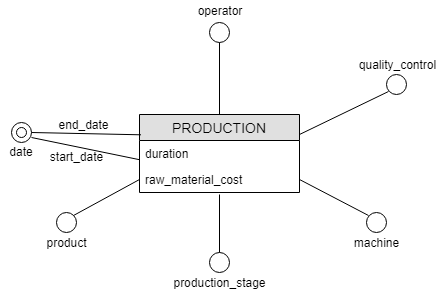
\includegraphics[scale=0.65]{../images/DFM_Production_Simple.png}
        \caption{
                \label{fig:production}  
                DFM of the production
        }
\end{figure}

\subsection{Showroom visit}

\begingroup
\renewcommand\arraystretch{0.5}
\begin{longtable}{p{4cm}p{9cm}}
        \caption{Fact table} \\
        Dimension & Attributes \\
        \endfirsthead \\
        Dimension & Attributes \\
        \endhead \\
        \hline \\
        Date & Day, Month, Year, Quartal, Week, Day of Week, Season, Holiday \\
        \hline \\
        Showroom & Name, City, District, Province, Region, Country, Manager, Address, Telephone, Size \\
        \hline \\
        Visitor & Name, City, District, Province, Region, Country, Language, Telephone, E-Mail, Type, Sector, Gender, Customer number \\
        \hline \\
        Order & Order Number, Total Price, Discount \\
        \hline \\
        Order Detail & Quantity, Quantity Type, Product, Unit price, Total price \\
        \hline \\
        Department & Name \\
        \hline \\
        Sales representative & Name, City, District, Province, Region, Country, Language, Telephone, E-Mail, Gender \\
        \hline \\
\end{longtable}
\endgroup

\begin{figure}[H] 
        \centering
        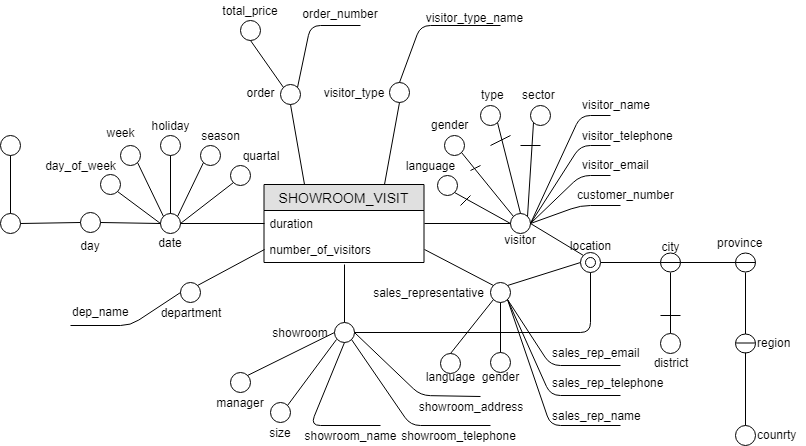
\includegraphics[width=\columnwidth]{../images/DFM_Showroom.png}
        \caption{
                \label{fig:showroomAttributes}  
                Dimension fact model (DFM) of the showroom visit with attributes 
        }
\end{figure}

\subsection{Production}

\begingroup
\renewcommand\arraystretch{0.5}
\begin{longtable}{p{4cm}p{9cm}}
        \caption{Fact table} \\
        Dimension & Attributes \\
        \endfirsthead \\
        Dimension & Attributes \\
        \endhead \\
        \hline \\
        Start date & Day, Month, Year, Week \\
        \hline \\
        End date & Day, Month, Year, Week \\
        \hline \\
        Product & Product number, Name, Department, Category \\
        \hline \\
        Production stage & Name \\
        \hline \\
        Machine & Name, Purchasing year, Vendor \\
        \hline \\
        Quality control & Grade \\
        \hline \\
        Operator & Name \\
        \hline \\
\end{longtable}
\endgroup

\begin{figure}[h] 
        \centering
        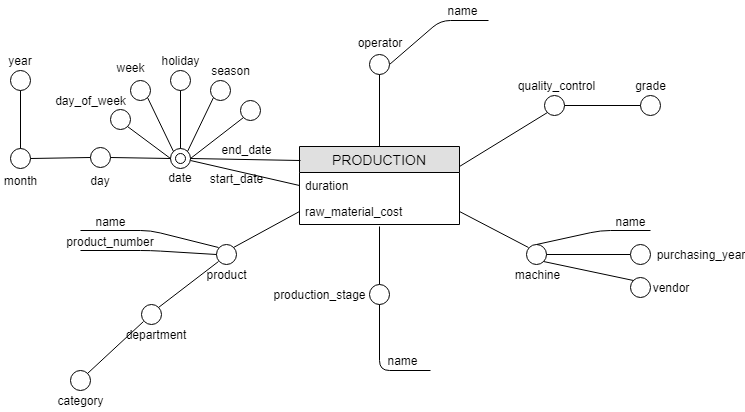
\includegraphics[width=\columnwidth]{../images/DFM_Production.png}
        \caption{
                \label{fig:productionAttributes}  
                Dimension fact model (DFM) of the production with attributes 
        }
\end{figure}

\section{Logical Design}

\subsection{Star schemas}

\begin{figure}[h] 
        \centering
        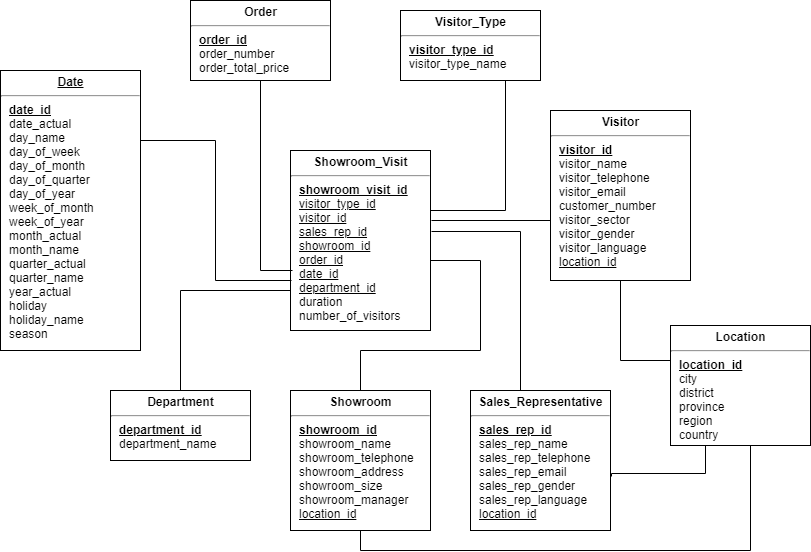
\includegraphics[width=\columnwidth]{../images/Starschema_Showroom_visit.png}
        \caption{
                \label{fig:starschemaShowroom}  
                Star schema of the showroom visit
        }
\end{figure}

\begin{figure}[h] 
        \centering
        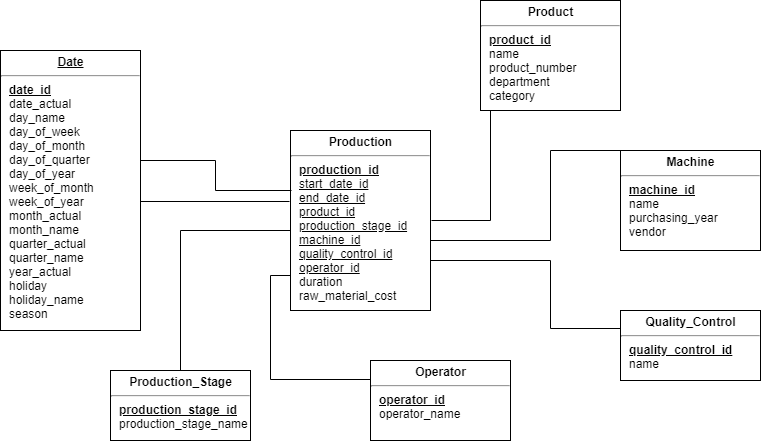
\includegraphics[width=\columnwidth]{../images/Starschema_Production.png}
        \caption{
                \label{fig:starschemaProduction}  
                Star schema of the production
        }
\end{figure}

\subsection{Two business questions}

\subsubsection{Fact: Showroom visit}

In order to be able to make the right marketing decisions, it is very important for the management to know from which sector the various customers or interested parties of a particular showroom come from. So, for example the management wants to know, from which sectors the various customers of showroom "Showroom-Bozen" were coming in the last year.

\bigskip
\noindent SQL query:
\begin{lstlisting}[
        language=SQL,
        showspaces=false,
        basicstyle=\ttfamily,
        numbers=left,
        numberstyle=\tiny,
        commentstyle=\color{gray}
     ]
SELECT v.visitor_sector, count(*)
FROM warehouse.visitor v
INNER JOIN warehouse.showroom_visit sv on v.visitor_id = sv.visitor_id
INNER JOIN warehouse.showroom s on sv.showroom_id = s.showroom_id
INNER JOIN warehouse.date d on sv.date_id = d.date_id
WHERE s.showroom_name = 'Showroom-BOZEN' 
AND d.date_actual >= '2018-01-01' AND d.date_actual <= '2018-12-31'
GROUP by v.visitor_sector
\end{lstlisting}

\begingroup
\renewcommand\arraystretch{0.5}
\begin{longtable}{p{1.4cm}p{1.5cm}p{1.8cm}p{1.5cm}p{1.6cm}p{1.4cm}p{1.2cm}p{1.25cm}p{1.85cm}}
        \caption{Showroom visit} \\
        ID & Visitor\_id & Sales\_rep\_id & Showr.\_id & Depart.\_id & Date\_id & Type\_id & Duration & Nr.\_of\_visit. \\
        \endfirsthead \\
        ID & Visitor\_id & Sales\_rep\_id & Showr.\_id & Depart.\_id & Date\_id & Type\_id & Duration & Nr.\_of\_visit. \\
        \endhead \\
        \hline \\
        1282369	& \color{red} 570822 & 6 & \color{red} 5 & 4 & \color{red}20180323 & 2 & 90 & 2 \\
        \hline \\
        1282370	& 570823 & 5 & 5 & 2 & 20160107 & 4 & 167 & 4 \\
        \hline \\
        1282371	& 570823 & 7 & 5 & 1 & 20130526 & 3 & 173 & 6 \\
        \hline \\
        1282372	& 570823 & 11 & 5 & 6 & 20150806  & 3 & 100 & 10 \\
        \hline \\
        1282373	& 570823 & 7 & 5 & 1 & 20121116 & 4 & 169 & 5 \\
        \hline \\
        1282374	& 570824 & 7 & 5 & 1 & 20171210 & 3 & 57 & 3 \\
        \hline \\
        1282375	& 570824 & 18 & 5 & 2 & 20110212 & 3 & 166 & 7 \\
        \hline \\
        1282376	& 570824 & 9 & 5 & 4 & 20130811  & 3 & 84 & 5 \\
        \hline \\
        1282377	& 570825 & 11 & 5 & 6 & 20170507 & 3 & 184 & 10 \\
        \hline \\
        1282378	& 570825 & 12 & 5 & 2 & 20111127 & 2 & 26 & 2 \\
        \hline \\
        1282379	& 570825 & 7 & 5 & 1 & 20150425 & 3 & 141 & 10 \\
        \hline \\
        1282380	& 570826 & 11 & 5 & 6 & 20130208 & 2 & 8 & 2 \\
        \hline \\
        1282381	& 570826 & 12 & 5 & 1 & 20111214 & 3 & 61 & 8 \\
        \hline \\
        1282382	& 570827 & 12 & 5 & 1 & 20170202 & 3 & 139 & 9 \\
        \hline \\
        1282383 & 570827 & 12 & 5 & 2 & 20121012 & 3 & 71 & 7 \\
        \hline \\
\end{longtable}
\endgroup

\begingroup
\renewcommand\arraystretch{0.5}
\begin{longtable}{p{1.3cm}p{1.6cm}p{1.8cm}p{3.6cm}p{2cm}p{.7cm}p{1.2cm}p{1.5cm}}
        \caption{Visitor} \\
        ID & Name & Telephone & E-Mail & Sector & Sex & Lang. & Loc.\_id \\
        \endfirsthead \\
        ID & Name & Telephone & E-Mail & Sector & Sex & Lang. & Loc.\_id \\
        \endhead \\
        \hline \\
        \color{red} 570822 & Melanie Eder &  &  & \color{red} Gastronomy & F & german & 9 \\
        \hline \\
        570823 & Julian Schmidt &  & j.schmidt@email.com & \color{red} Private & M & german & 9 \\
        \hline \\
        570824 & Marcel Schwarz & 306 9579783 & m.schwarz@email.com & \color{red} Hotel & M & german & 9 \\
        \hline \\
        570825 & Denise Fuchs & 396 5305260 & d.fuchs@email.com & \color{red} Public & F & german & 9 \\
        \hline \\
        570826 & Sophie Wimmer & 322 7641804 & s.wimmer@email.com & \color{red} Private & F & german & 9 \\
        \hline \\
\end{longtable} 
\endgroup

\begingroup
\renewcommand\arraystretch{0.5}
\begin{longtable}{p{0.25cm}p{3.9cm}p{2.2cm}p{2.9cm}p{.7cm}p{3.1cm}p{1.1cm}}
        \caption{Showroom} \\
        ID & Name & Telephone & Address & Size & Manager & Loc.\_id \\
        \endfirsthead \\
        ID & Name & Telephone & Address & Size & Manager & Loc.\_id \\
        \endhead \\
        \hline \\
        1 & Showroom-LATSCH & 0477 069655 & Herrengasse 8 & 581 & Paul Wolf & 42 \\
        \hline \\
        2 & Showroom-M{\"U}HLBACH & 0474 039227 & Platzerstr. 58 & 349 & Christoph Steiner & 54 \\
        \hline \\
        3 & Showroom-M{\"O}LTEN & 0470 429676 & Vernag 97 & 857 & Christoph Steiner & 51 \\
        \hline \\
        4 & Showroom-SALURN & 0475 248487 & Gewerbezone 44 & 198 & Johannes Egger & 77 \\
        \hline \\
        \color{red} 5 & \color{red} Showroom-BOZEN & 0473 723301 & St. Urban 73 & 447 & Sabine Schneider & 9 \\
        \hline \\
\end{longtable} 
\endgroup

\begingroup
\renewcommand\arraystretch{0.5}
\begin{longtable}{p{1.6cm}p{2.1cm}p{1.4cm}p{1.5cm}p{1.6cm}p{1cm}p{1cm}p{1.1cm}p{1.2cm}}
        \caption{Date} \\
        ID & Date & Day\_week & Day & Month & Quartal & Year & Holiday & Season \\
        \endfirsthead \\
        ID & Date & Day\_week & Day & Month & Quartal & Year & Holiday & Season \\
        \endhead \\
        \hline \\
        20160102 & 2010-01-02 & 6 & Saturday & January & First & 2016 & false & Winter \\
        \hline \\
        20170103 & 2010-01-03 & 7 & Sunday & January & First & 2017 & false & Winter \\
        \hline \\
        20180108 & \color{red} 2018-01-08 & 5 & Friday & January & First & 2018 & false & Winter \\
        \hline \\
        20190109 & 2010-01-09 & 6 & Saturday & January & First & 2019 & false & Winter \\
        \hline \\
        20200110 & 2010-01-10 & 7 & Sunday & January & First & 2020 & false & Winter \\
        \hline \\
\end{longtable} 
\endgroup

\begingroup
\renewcommand\arraystretch{0.5}
\begin{longtable}{p{3cm}p{4cm}}
        \caption{Result of the query} \\
        Sector & Number of visitors \\
        \endfirsthead \\
        Sector & Number of visitors \\
        \endhead \\
        \hline \\
        Gastronomy & 2985 \\
        \hline \\
        Hotel & 4223 \\
        \hline \\
        Private & 5629 \\
        \hline \\
        Public & 1371 \\
        \hline \\
\end{longtable} 
\endgroup

\subsubsection{Fact: Production}

The company's quality control is always interested in optimizing processes. It is therefore interesting for employees to know whether a machine has significant time differences in production in relation to a particular product in comparison to the other machines.

\bigskip
\noindent SQL query:
\begin{lstlisting}[
        language=SQL,
        showspaces=false,
        basicstyle=\ttfamily,
        numbers=left,
        numberstyle=\tiny,
        commentstyle=\color{gray}
     ]
SELECT m.machine_name, avg(p.duration) AS avg_production_duration
FROM warehouse.machine m
INNER JOIN warehouse.production p ON m.machine_id = p.machine_id
INNER JOIN warehouse.product o ON p.product_id = o.product_id
WHERE o.product_number = 'Warteraum-Couch - 10'
GROUP BY m.machine_id
ORDER BY avg_production_duration DESC LIMIT 10
\end{lstlisting}

\begingroup
\renewcommand\arraystretch{0.5}
\begin{longtable}{p{1cm}p{1.5cm}p{1.5cm}p{1cm}p{1.5cm}p{1.8cm}p{1.6cm}p{1.3cm}p{2.2cm}}
        \caption{Production} \\
        ID & Operator* & Machine* & Stage* & Product* & Start\_date* & End\_date* & Duration & Raw\_mat.\_cost \\
        \endfirsthead \\
        ID & Operator* & Machine* & Stage* & Product* & Start\_date* & End\_date* & Duration & Raw\_mat.\_cost \\
        \endhead \\
        \hline \\
        591814 & 779 & 1144 & 1 & \color{red} 361016 & 20101105 & 20101202 & 152 & 76 \\
        \hline \\
        591815 & 780 & 1174 & 2 & \color{red} 361016 & 20101202 & 20101203 & 1 & 395 \\
        \hline \\
        591816 & 775 & 1213 & 3 & \color{red} 361016 & 20101203 & 20101207 & 2 & 277 \\
        \hline \\
        591817 & 770 & 1055 & 1 & \color{red} 361016 & 20101122 & 20101214 & 30 & 66 \\
        \hline \\
        591818 & 722 & \color{red} 1176 & 2 & \color{red} 361016 & 20101214 & 20110111 & 133 & 391 \\
        \hline \\
        591819 & 755 & 1079 & 3 & \color{red} 361016 & 20110111 & 20110204 & 36 & 275 \\
        \hline \\
        591820 & 740 & 1069 & 1 & \color{red} 361016 & 20150511 & 20150520 & 49 & 73 \\
        \hline \\
        591821 & 756 & 1025 & 2 & \color{red} 361016 & 20150520 & 20150603 & 54 & 398 \\
        \hline \\
        591822 & 758 & 1130 & 3 & \color{red} 361016 & 20150603 & 20150625 & 96 & 278 \\
        \hline \\
        27064 & 754 & 1164 & 1 & \color{red} 361016 & 20101022 & 20101026 & 8 & 66 \\
        \hline \\
        27065 & 739 & 1028 & 2 & \color{red} 361016 & 20101026 & 20101104 & 6 & 407 \\
        \hline \\
        27066 & 798 & 1098 & 3 & \color{red} 361016 & 20101104 & 20101105 & 6 & 280 \\
        \hline \\
        27067 & 780 & 1013 & 1 & \color{red} 361016 & 20130327 & 20130411 & 70 & 74 \\
        \hline \\
        27068 & 737 & 1145 & 2 & \color{red} 361016 & 20130411 & 20130509 & 18 & 404 \\
        \hline \\
        27069 & 772 & 1032 & 3 & \color{red} 361016 & 20130509 & 20130520 & 14 & 281 \\
        \hline \\
\end{longtable} 
\endgroup

Note: all columns with the * are foreign key columns and are carrying only the id

\begingroup
\renewcommand\arraystretch{0.5}
\begin{longtable}{p{1cm}p{3cm}p{3.2cm}p{3.1cm}}
        \caption{Machine} \\
        ID & Machine\_name & Machine\_vendor & Purchasing\_year \\
        \endfirsthead \\
        ID & Machine\_name & Machine\_vendor & Purchasing\_year \\
        \endhead \\
        \hline \\
        1172 & Melichár & Durán & 1998 \\
        \hline \\
        1173 & Horn & Λόντος & 2009 \\
        \hline \\
        1174 & Chihaia & Murtazaev & 2002 \\
        \hline \\
        1175 & Korčák & Durán & 2006 \\
        \hline \\
        \color{red} 1176 & \color{red} Ramóna & Barbora & 1996 \\
        \hline \\
\end{longtable} 
\endgroup

\begingroup
\renewcommand\arraystretch{0.5}
\begin{longtable}{p{3cm}p{4cm}}
        \caption{Result of the query} \\
        Machine\_name & AVG\_Production\_duration \\
        \endfirsthead \\
        Machine\_name & AVG\_Production\_duration \\
        \endhead \\
        \hline \\
        Vajda & 152.00 \\
        \hline \\
        \color{red} Ramóna & 133.00 \\
        \hline \\
        Παπανδρέου & 96.00 \\
        \hline \\
        Κοντολέων & 70.00 \\
        \hline \\
        Mitu & 54.00 \\
        \hline \\
        Bercu & 49.00 \\
        \hline \\
        Heinrich & 36.00 \\
        \hline \\
        Martinez & 30.00 \\
        \hline \\
        Pál & 18.00 \\
        \hline \\
        Aguilar & 14.00 \\
        \hline \\
\end{longtable} 
\endgroup

\section{Conclusions}


\bibliography{references}{}
\bibliographystyle{plain}

\end{document}